\documentclass{article}

\usepackage{amsmath}
\usepackage{amsfonts} % For math fonts.
\usepackage{amssymb} % For other math symbols not covered by amsmath.
\usepackage[pdftex]{graphicx} % For pictures, use \includegraphics[scale=decimal]{pic.png}; must be a .png file type.
\usepackage{multicol}
\usepackage{textcomp}
\usepackage[colorlinks = true, urlcolor = blue]{hyperref}
\usepackage{enumitem}
\usepackage{graphbox} 
\usepackage{subfig}
\usepackage{multicol}
\usepackage{nopageno}


\usepackage{tikz}
\usetikzlibrary{positioning, calc}
\usetikzlibrary{shapes.geometric,angles,quotes}
\usepackage{tikz-3dplot}


%page formatting
\usepackage{fullpage}
\setlength{\parindent}{0pt}


\newcommand{\tab}{\hspace*{0.25in}}
\newcommand{\csq}[1]{\reflectbox{''}#1''}  %This produces CS style quotes.
\newcommand{\csqt}[1]{\text{\reflectbox{''}#1''}}  %This produces CS style quotes as text.


\usepackage{listings}
\lstset
{ %Formatting for code in appendix
    language=Python,
    basicstyle=\footnotesize,
    numbers=left,
    stepnumber=1,
    showstringspaces=false,
    tabsize=2,
    breaklines=true,
    breakatwhitespace=false,
}


\begin{document}



%split_point

%\end{document}
Matt Priem \hfill midterm retake quiz\\
section 1\\
\begin{enumerate}
	\item 
		(Game: heads or tails)  Write a program that lets the user guess whether the flip of a coin 
		results in heads or tails.  The program randomly generates an integer 0 or 1, which 
		represents head or tail.  The program prompts the user to enter a guess and reports whether 
		the guess is correct or incorrect.\\
		Hint: These should be your first two lines of code.
		\begin{verbatim}
		    from random import randint
		    value = randint(0,1) #picks a random integer. Either 0 or 1.
		\end{verbatim}



	\item
		Write a program that asks the user for three numbers, and then determines (and outputs) which of the 
		numbers is the smallest.  Do not use the built-in function \textit{min}().\\
		For example, \\ \ \hfill
		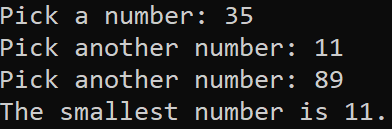
\includegraphics[height = 0.6in]{./imgs/smallest_ex1.PNG} \hfill
		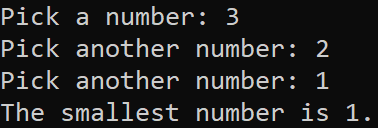
\includegraphics[height = 0.6in]{./imgs/smallest_ex2.PNG} \hfill \ 




	\item 
		%https://edabit.com/challenge/xR248CxGSsSrNK5Za
		You are the newest rug fashion designer on the scene, but you're running out of ideas. 
		Write a program that will help you design rugs.  The program should ask for a width, 
		a length, and pattern, and then create a rug consisting of that pattern and dimensions.

		For example, \\ \ \hfill
		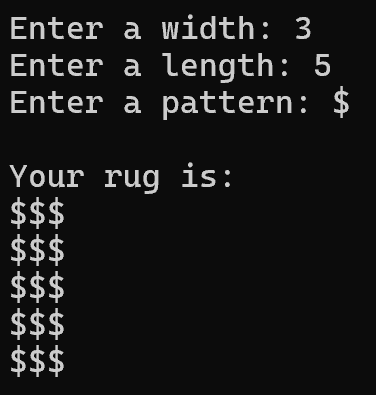
\includegraphics[width = 1.5in]{./imgs/rug1.PNG} \hfill  
		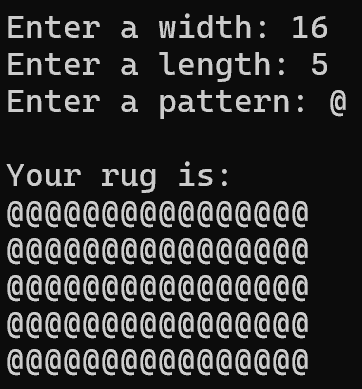
\includegraphics[width = 1.5in]{./imgs/rug2.PNG} \hfill \


	\item 
		Using a loop, write a program that prints every even number 
		between 37 and 1050 (inclusively).


	\item 
		%https://edabit.com/challenge/Ay9wPrqRJnBmvbFmi
		Ask the user for two integers named \textit{larger} and \textit{smaller}.  Determine (and output) 
		how many times larger can be halved while still be greater than smaller.
		
		Examples:
		\begin{itemize}
			\item if \textit{larger} = 1324 and  \textit{smaller} = 98, the result should be 3 since
				1324 $\rightarrow$ 662 $\rightarrow$ 331 $\rightarrow$ 165.5
			\item if \textit{larger} = 624 and  \textit{smaller} = 8, the result should be 6 since\\
				\tab 624 $\rightarrow$ 312 $\rightarrow$ 156 $\rightarrow$ 78 $\rightarrow$ 39 
				$\rightarrow$ 19.5 $\rightarrow$ 9.75)
		\end{itemize}


\end{enumerate}
\pagebreak
Bart Simpson \hfill midterm retake quiz\\
section 1\\
\begin{enumerate}
	\item 
		Using a loop, write code to calculate the sum of all odd numbers between 50 and 517. 
		Print the result.


	%new
	\item 
		At the local coffee shop they have 3 types of coffee, which are Espresso, Latte, and Cappuccino.  
		Write a \textbf{function} that returns the selected coffee type. If the chosen type is not available, let them know.
		The argument to the function will be $selected\_coffee$ (the user's selected coffee type).\\
		\textbf{Examples:}		
		\begin{itemize}
			\item  serve\_coffee(\csq{Latte}) $\rightarrow$ \csq{Here is your latte!}, 
			\item  serve\_coffee(\csq{Mocha}) $\rightarrow$ \csq{Sorry, we don't have mocha.}, 
			\item  serve\_coffee(\csq{Espresso}) $\rightarrow$ \csq{Here is your espresso!}
		\end{itemize}


	\item 
		%https://edabit.com/challenge/nfWirHJzNRBMAp9Df
		The \textbf{hamming distance} is the number of characters that differ between two strings.\\
		To illustrate, \\ \hspace*{1em}
		\begin{tabular}{lll}
			str1 = &\csq{abcbba}\\
			str2 = &\csq{abcbda}
		\end{tabular}\\
		The hamming distance is 1 since the only difference is the $5^{th}$ character. \\ 
		That is, \csq{b} in str1 vs. \csq{d} in str2.
		
		Your task: create a function named hamming distance that takes two strings as arguments, 
		and returns the hamming distance between the two strings.

	\textbf{Examples:}
		\begin{itemize}
			\item hamming\_distance(\csq{abcde}, \csq{bcdef}) $\rightarrow$ 5, 
				since all 5 letters are different.
			\item hamming\_distance(\csq{abcdef}, \csq{abcdef}) $\rightarrow$ 0, 
				since all 6 letters are the same.
			\item hamming\_distance(\csq{strong}, \csq{strung}) $\rightarrow$ 1,
				since there is only 1 character that is different.
		\end{itemize}

\end{enumerate}
\pagebreak
Dot Matrix \hfill midterm retake quiz\\
section 3\\
\begin{enumerate}
	\item 
		Write a program that asks the user for \\
		\begin{minipage}{0.5\textwidth}
		\vspace*{-0.5em}
			\begin{enumerate}  \setlength\itemsep{-0.3em}
				\item a food and
				\item a drink.  
			\end{enumerate} \vspace*{-1ex}
		and then outputs their order.
		\end{minipage}
		%\
		\begin{minipage}{0.5\textwidth}
			\centering
			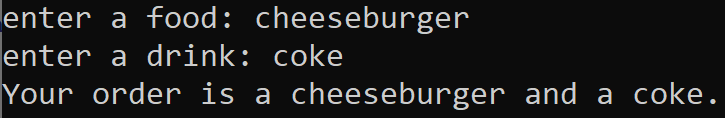
\includegraphics[scale=0.75]{./imgs/outputFoodAndDrink.png}\\
			Your output should be similar to this.
		\end{minipage}



	%paper-based
	\item 	
		Below is a receipt from my recent lunch order.
		\begin{enumerate}
			\item Initialize an empty dictionary named receipt, and then add the contents of 
				the receipt as key-value pairs.
			\item Using the dictionary you created in part a, write code that prints the 
				total cost of all the items on the receipt.  The code should work regardless
				of the contents of the receipt. (meaning don't write print(6+12+3))
		\end{enumerate}	
		\begin{center}
		        \begin{tabular}{l|c}
		            \textbf{Item} & \textbf{Price} \\ \hline
		            Side Salad & \$6 \\
		            Chicken Parm & \$12 \\
		            Cookie & \$3 \\
		        \end{tabular}
		\end{center}

	%paper-based
	\item 	
		Write a \textbf{function} that takes a string $word$ and returns a dictionary containing the count of each letter in the word. 

		\textbf{Examples:}		
		\begin{itemize}
			\item  letter\_count(\csq{hello}) $\rightarrow$ \{\csq{h}: 1, \csq{e}: 1, \csq{l}: 2, \csq{o}: 1\}
			\item  letter\_count(\csq{mississippi}) $\rightarrow$ \{\csq{m}: 1, \csq{i}: 4, \csq{s}: 4, \csq{p}: 2\}
			\item  letter\_count(\csq{apple}) $\rightarrow$ \{\csq{a}: 1, \csq{p}: 2, \csq{l}: 1, \csq{e}: 1\}
		\end{itemize}


	%new
	\item 
		Write a \textbf{function} that loops through and prints every even number between two
		integers (inclusive). The arguments to the function will be $smaller\_num$ and 
		$larger\_num$.

		\textbf{Examples:}		
		\begin{itemize}
			\item  output\_even(37, 1050) $\rightarrow$ 38, 40, 42, \dots 1048, 1050, 
			\item  output\_even(1, 2000) $\rightarrow$ 2, 4, 6, \dots 1998, 2000 
			\item  output\_even(50, 199) $\rightarrow$ 50, 52, 54, \dots 196, 198
		\end{itemize}


	\item 	
		%https://edabit.com/challenge/vTGXrd5ntYRk3t6Ma
		An isogram is a word that has no duplicate letters. Write a \textbf{function} that takes a string $word$ 
		and returns either True or False depending on whether or not it's an isogram.

		\textbf{Examples:}		
		\begin{itemize}
			\item  is\_isogram(\csq{algorism}) $\rightarrow$ True
			\item  is\_isogram(\csq{password}) $\rightarrow$ False
			\item  is\_isogram(\csq{consecutive}) $\rightarrow$ False
		\end{itemize}


\end{enumerate}
\pagebreak
Alfred Yankovic \hfill midterm retake quiz\\
section 2\\
\begin{enumerate}
	\item 
		Write a program for an agreeable AI.\\
		The computer should ask the user for \\
		\begin{minipage}{0.5\textwidth}
		\vspace*{-0.5em}
			\begin{enumerate}  \setlength\itemsep{-0.3em}
				\item a color and
				\item a food.  
			\end{enumerate} \vspace*{-1ex}
		and then outputs their order.
		\end{minipage}
		%\
		\begin{minipage}{0.5\textwidth}
			\centering
			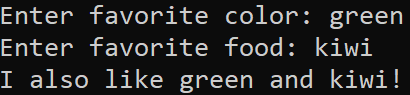
\includegraphics[scale=0.75]{./imgs/agreeableAIoutput.png}\\
			Your output should be similar to this.
		\end{minipage}


	\item Write a program that asks the user for \\
		\begin{minipage}{0.5\textwidth}	
		\vspace*{-0.5em}
			\begin{enumerate}  \setlength\itemsep{-0.3em}
				\item the year,
				\item the month, and
				\item the day	
			\end{enumerate} \vspace*{-1ex}
		and then outputs the date.
		\end{minipage}
		%\
		\begin{minipage}{0.5\textwidth}
			\centering
			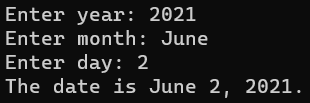
\includegraphics[scale=0.75]{./imgs/dateOutput.png}\\
			Your output should be similar to this.
		\end{minipage}

	


	\item 
		Write a program that prompts the user to enter three integers and displays the integers 
		in decreasing order (largest to smallest).  You may not use the built-in functions 
		\textit{max}(), \textit{min}(), \textit{sort}() or \textit{sorted}().


	\item 
		At the local ice cream store they have 3 flavors, which are Vanilla, Chocolate, and Strawberry.  
		Write a \textbf{function} that returns the selected flavor. If the chosen flavor is not available, let them know.
		The argument to the function will be $selected\_flavor$ (the user's selected flavor).\\
		\textbf{Examples:}		
		\begin{itemize}
			\item  serve\_icecream(\csq{Vanilla}) $\rightarrow$ \csq{Here is your vanilla ice cream!}, 
			\item  serve\_icecream(\csq{Mint}) $\rightarrow$ \csq{Sorry, we don't have mint ice cream.}, 
			\item  serve\_icecream(\csq{Chocolate}) $\rightarrow$ \csq{Here is your chocolate ice cream!} 
		\end{itemize}


\end{enumerate}
\pagebreak
\end{document}